\documentclass[]{article}
\usepackage{graphicx}
\usepackage{float}
\usepackage{amsmath}
%\usepackage[]{hyperref}
% Title Page
\title{Lab 3}
\author{
	Alex Taglieri
	\\
	Andrew Kacherski
	}

\begin{document}
\maketitle
\newpage
\
\raggedright


\pagenumbering{arabic}
\section{Introduction and Background}

This lab explores the relationship between the idealized mass-spring system, where the spring's mass is assumed to be 0, and a more realistic model where the spring does have mass.

The general formula for the uncertainty of $ \omega $ is given by the following equation:


\begin{equation}\label{uncertaintyLong}
\Delta \omega = \frac{1}{2}(\sqrt{\frac{1}{mk}}\Delta k - \sqrt{\frac{k}{m^3}}\Delta m)
\end{equation}

In this case, dividing $ \frac{\Delta \omega}{\omega} $ gives

\begin{equation}\label{uncertainty}
\frac{\Delta \omega}{\omega} = \frac{1}{2} \left\| \frac{\Delta k}{k} \right\|+ \frac{1}{2} \left\|\frac{\Delta m}{m} \right\|
\end{equation}


The reason we are doing this is to prove that ignoring the mass of the spring cannot always be done so simply. 

\section{Procedure}

The general strategy for this lab is similar to the one followed in labs 1 and 2: find the \textit{k}-value for both kinds of springs when they're not moving, and then find their \textit{k}-values when they're oscillating.

There are two springs that will be used in this lab: one is a thin one, and one is a thick one. The thin one's mass is 3.6g, and the thick one's mass is 6.2g.

Hang 100g of mass from the scale and zero the readings of both the force sensor and the distance sensor. Add mass in 100g increments until reaching 600g, recording measurements at each step. Repeat for both the thin spring and the thick spring.

Then reduce the mass to 300g for the thin spring, or 400g for the thick spring, set the whole system in purely vertical motion, and tell the computer to track the system's position and force.


\section{Results}

The thin spring had a \textit{k}-value of 33.16 N/m. The masses were within \textit{0.5g} of their expected mass. The thick spring had a resultant k-value of 32.81 N/m. 

The angular frequency observed for the thin spring was 10.43 rad/sec with an uncertainty of 0.0003 rad/sec, and the angular frequency for the thick spring was 9.044 rad/sec with an uncertainty of 0.0002938 rad/sec.

The uncertainty measured for the 300g mass (when oscillating) was .00018 g. The uncertainty measured for the 400g mass (also when oscillating) was .0001723g.

The uncertainty measured for the thin spring's \textit{k}-value was 0.1909 N/m, and the uncertainty measured for the thick spring was .06505 N/m.


\begin{figure}[H]
	\centering
	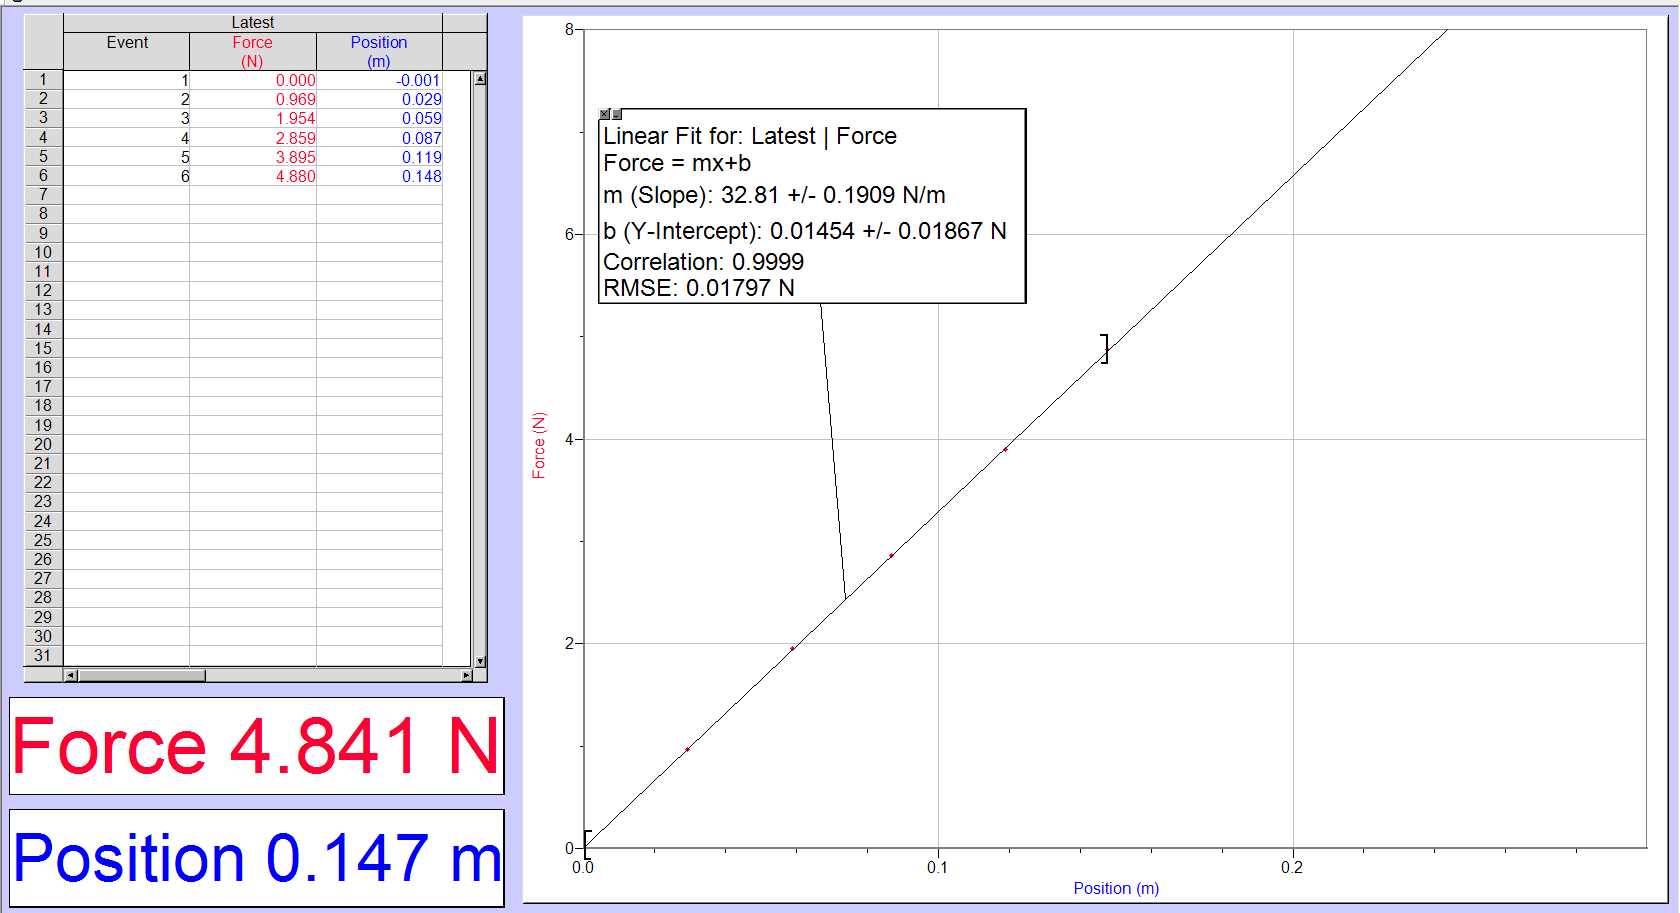
\includegraphics[width=\textwidth]{res/p1thinSpring}
	\caption{Thin Spring}
	\label{fig:Thin Spring}
\end{figure}

\begin{figure}[H]
	\centering
	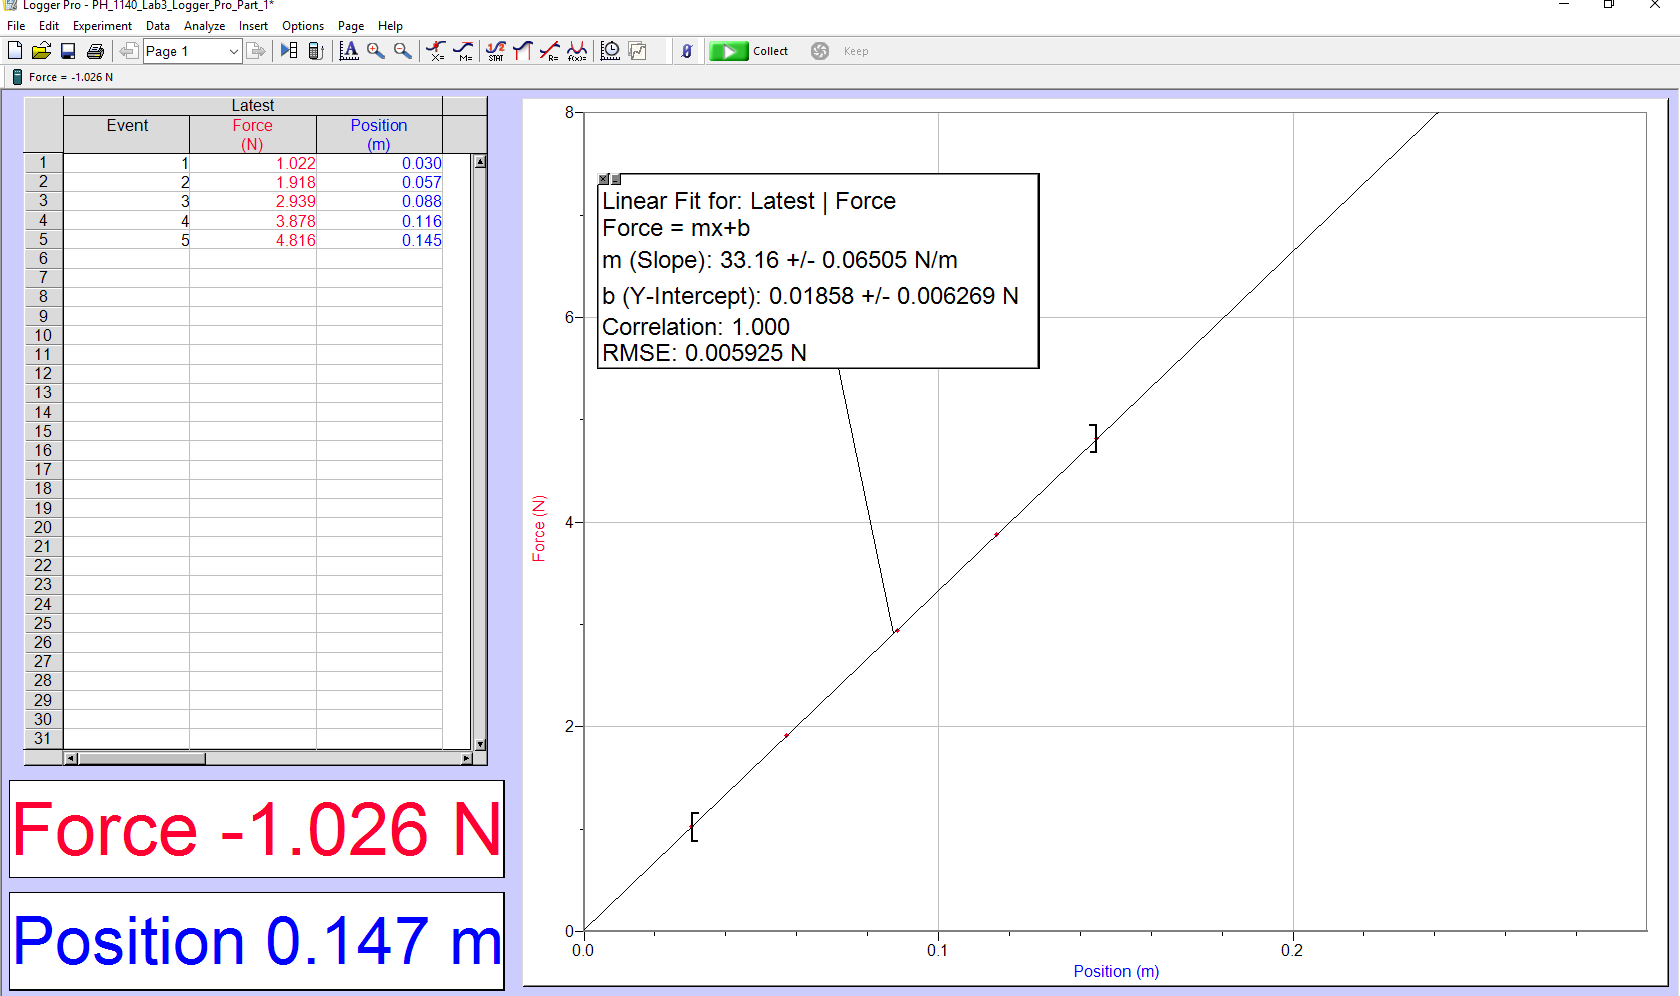
\includegraphics[width=\textwidth]{res/p1fatSpring}
	\caption{Thick Spring}
	\label{fig:Thick Spring}
\end{figure}

\begin{figure}[H]
	\centering
	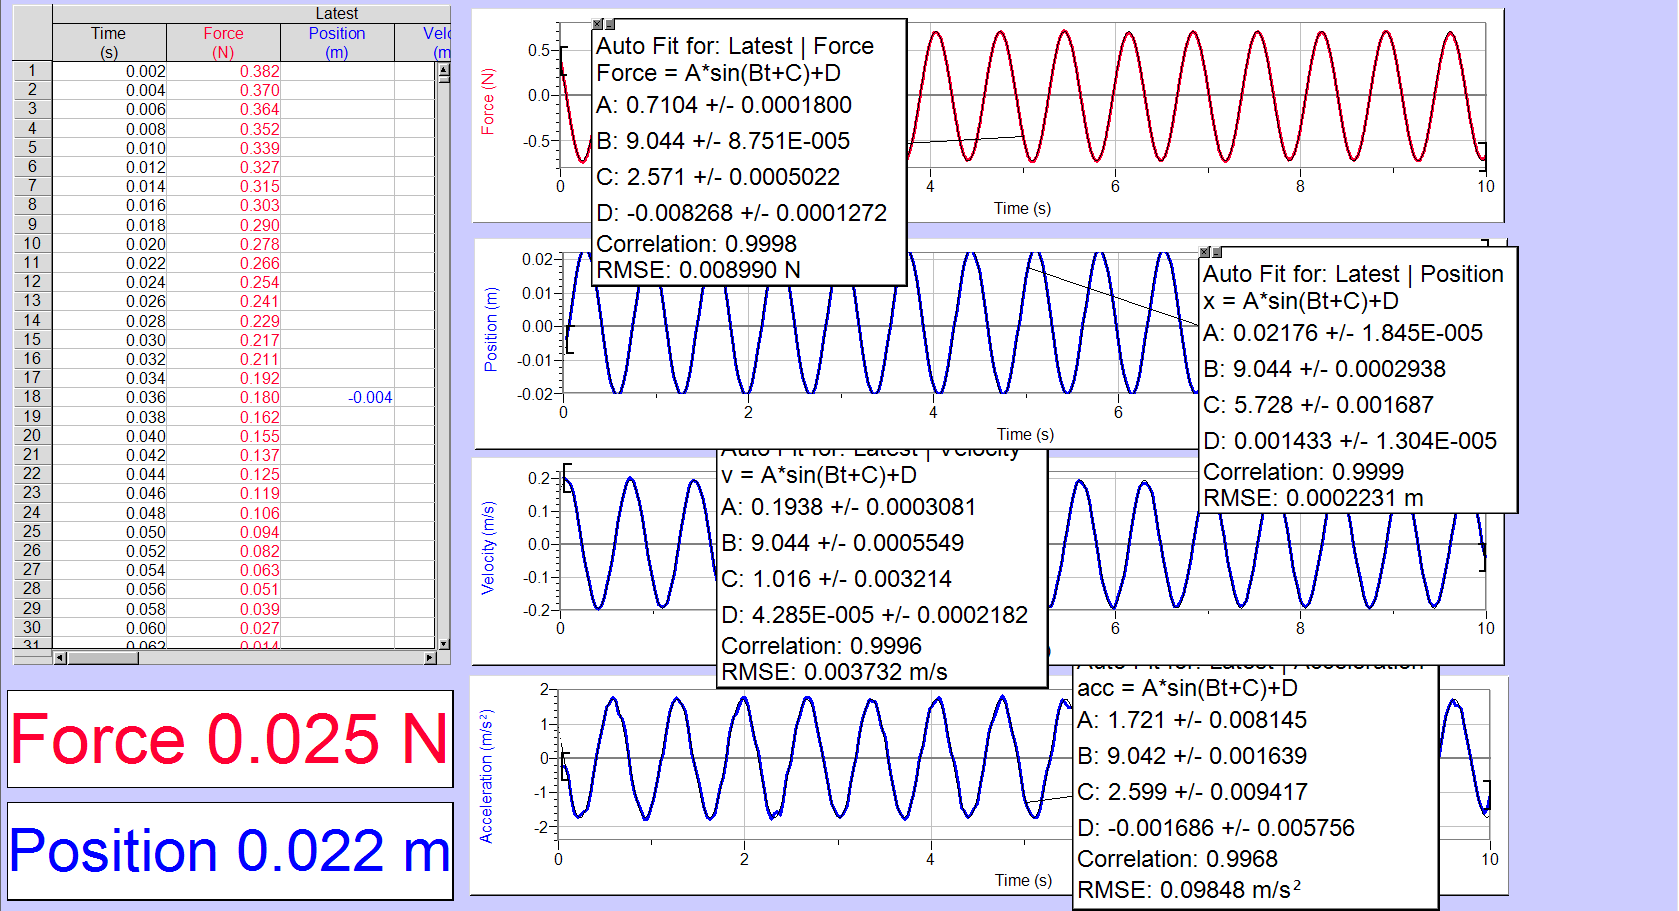
\includegraphics[width=\textwidth]{res/p2_400g}
	\caption{Oscillation with Thin Spring}
	\label{fig:Oscillation with Thin Spring}
\end{figure}

\begin{figure}[H]
	\centering
	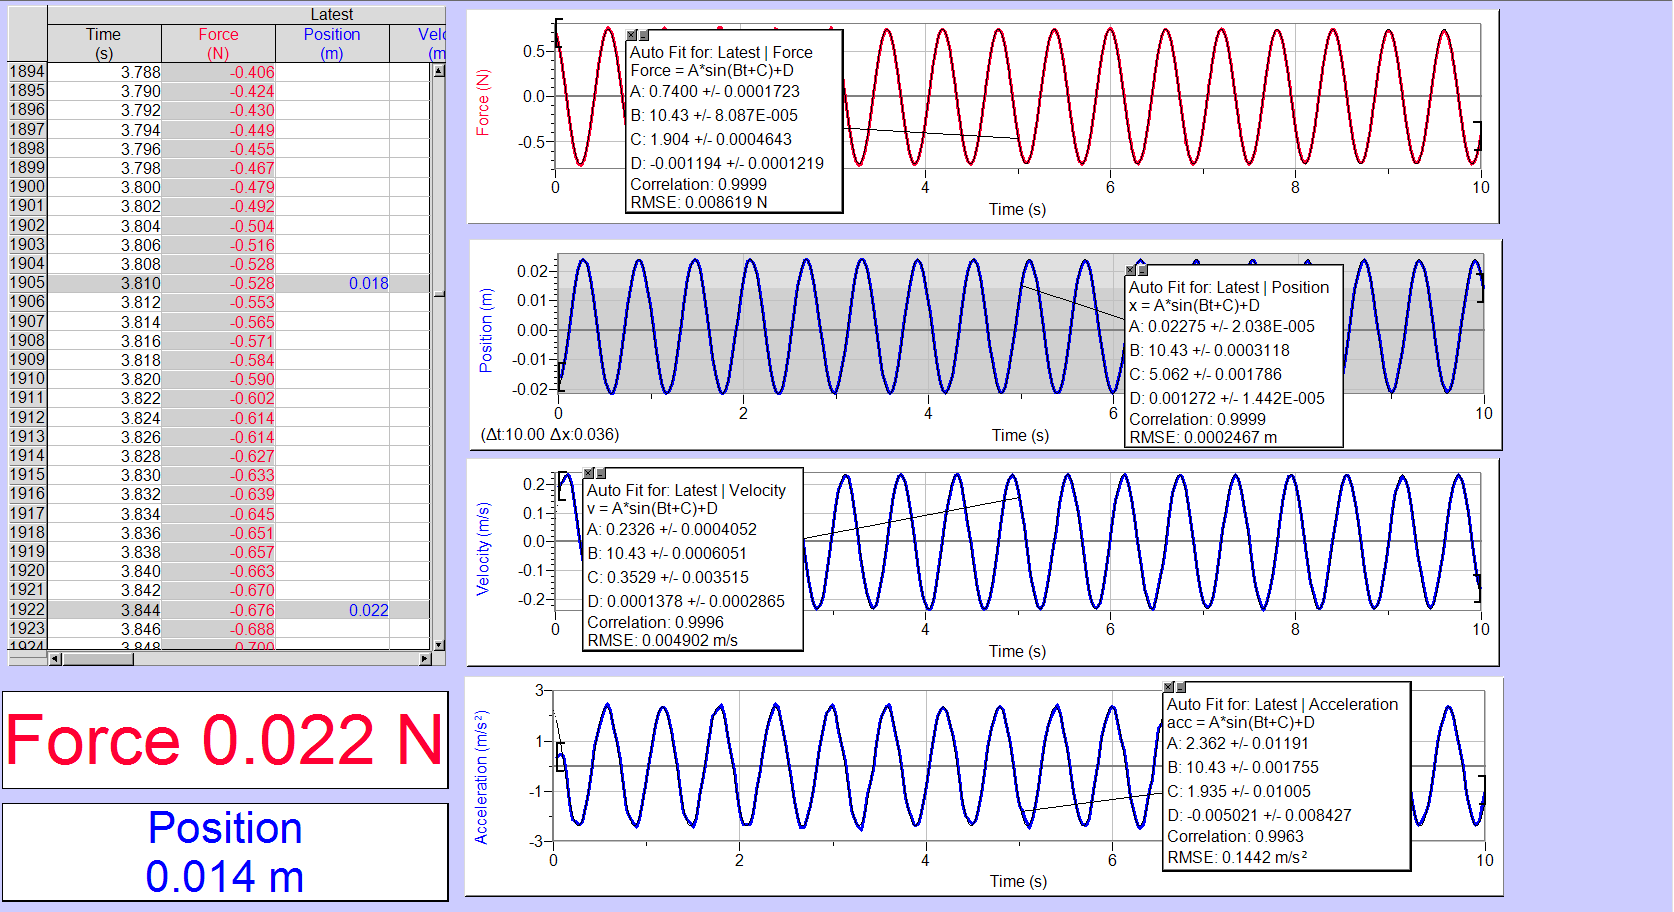
\includegraphics[width=\textwidth]{res/p2_thinSpring}
	\caption{Oscillation with Thick Spring}
	\label{fig:Oscillation with Thick Spring}
\end{figure}


\section{Discussion}

In the Results section, we found the uncertainties of k and m, and consequently the uncertainties of the $ \omega $'s. Here we'll plug them into the equation from the Background section.

The equation above is reproduced here:

\begin{equation}\label{uncertainty}
\frac{\Delta \omega}{\omega} = \frac{1}{2} \left\| \frac{\Delta k}{k} \right\|+ \frac{1}{2} \left\|\frac{\Delta m}{m} \right\|
\end{equation}

Plugging in:

\begin{equation}\label{uncertainty}
\begin{split}
\frac{\Delta \omega}{9.044} &= \frac{1}{2} \left\| \frac{0.1909}{33.16} \right\|+ \frac{1}{2} \left\|\frac{.00018}{300} \right\| \\
&= 0.002878768 -> \Delta \omega = 0.026035578 Rad / sec
\end{split}
\end{equation}

$ \Delta \omega $ was .0000875 according to our measurements. We attribute this error to the fact that both $ \Delta k $ and $ \Delta m $ were measured with only 4 data points, while $ \Delta \omega $ was measured with a few orders of magnitude more data points. The same is true of the thick spring.


\end{document}          
